\documentclass[11pt]{amsart}

\usepackage{macros, setspace}
\usepackage{hyperref}
\usepackage{amsmath,amsthm}

\author{Natalie M. Paquette and Brian R. Williams}
\date{\today}
\title{Koszul duality in QFT}

\def\define{\overset{\rm def}{=}}
\def\ep{\varepsilon}
\def\zbar{{\overline{z}}}
\def\Weyl{{\rm Weyl}}
\def\Cl{{\rm C}\ell}
\def\U{{\rm U}}

\def\brian#1{{\textcolor{blue!65!red}{BRW: {#1}}}}
\def\natalie#1{{\textcolor{green!65!black}{BRW: {#1}}}}

\usepackage[upint]{stix}

\begin{document}
\maketitle

\spacing{1.25}

\section{Introduction}

\section{A biased review of Koszul duality} 

%sym and alt
%maybe a few words about mapping of modules btw derived categories? how does this relate to the line picture?
%CE(g) and U(g)

\subsection{Commutative-Lie duality}

%CE complex

\subsection{Associative-Associative duality} 

%hochschild

\subsection{A look at $\EE_n$ Koszul duality}

\subsection{Deformed Koszul duality}

\section{QFT rudiments}
%clarify: algebra of local ops vs. dense inclusion we work with in practice?

%Explain our conventions/some basic facts about the cohomological degree as ghost number, as well as the meaning of various degree shifts, which are unfamiliar to most physicists. 

\subsection{Local functionals and Maurer--Cartan elements} 



\subsection{Local operators}

Let $\Obs$ be the local operators of a one-dimensional translation invariant theory, and let $Q$ denote the BRST operator which acts on the theory.
The infinitesimal action by translations is through the time derivative $\frac{\partial}{\partial t}$. 

A one-dimensional theory is topological if there exists an endomorphism $\hat{Q}$ of the local operators, of cohomological degree $-1$, which satisfies
\[
\{Q, \hat{Q}\} = \frac{\partial}{\partial t} .
\]
In words, translations along the line are trivial in BRST cohomology. 
%Should we here contrast with notion of topological QFT coming from Q-exact stress tensors, which is a stronger statement?

%To be clarified: even ignoring BV/BRST extensions, we often have the freedom to enlarge the basic space of fields (dual to ops). E.g. U(1) gauge theory in the first order formalism enlarges from (gauge fields) to (gauge fields) x \Omega^{d-2}(M)... how is Koszul duality insensitive to this?

\subsection{Topological descent} 

Let $\Obs$ be the local operators of a one-dimensional topological field theory on $\RR$. 
Because the theory is translation invariant, we can consider the complex of {\em differential form} valued operators
\[
\Omega^\bu(\RR \, , \, \Obs) .
\]
This complex is equipped with the original BRST differential $Q$ acting on $\Obs$ as well as the de Rham differential $\d$. 

Given a local 0-form operator, $\cO = \cO^{(0)} \in \Obs$, we can use the endomorphism $\hat{Q}$ to define the following one-form valued operator
\[
\cO^{(1)} \define (\hat{Q} \cdot \cO) \d t \in \Omega^1(\RR \, , \, \Obs).
\]
The inhomogenous operator $\cO^{(0)} + \cO^{(1)}$ is closed in $\Omega^\bu(\RR \, , \, \Obs)$ if and only if the following descent equations are satisfied 
\begin{align*}
Q \cO^{(0)} & = 0 \\
\d \cO^{(0)} + Q \cO^{(1)} & = 0 .
\end{align*}

Topological descent equations were first explored by Witten in the Donaldson twist of 4d $\cN=2$ theory \cite{W88} as a means to obtain smeared gauge-invariant observables from local operators of higher ghost number. The solutions to the descent equations were constructed more generally in \cite{MW97}; they may also be familiar to string theorists from their application to the BRST cohomology of noncritical string theories, e.g. \cite{WZ92}. 

In particular, if $\{Q,\cO^{(0)}\} = 0$ then $\cO^{(1)}$ defines the following $Q$-closed local functional
\[
\int_{\RR} \cO^{(1)} .
\]
The superscript denotes a 1-form operator, now in cohomological degree (ghost number) 0, as appropriate for a gauge-invariant term in the Lagrangian. 


\subsection{Vacuums and augmentations}

%discrete choices of vacua vs. moduli spaces of vacua

\section{Line operators}

%universal line defects and Koszul duality
%stress relationship between three perspectives: MC(AxB), Hom(A!, B), couplings as local functionals from descent

\subsection*{Topological mechanics}

%free fermions/bosons in CS example? In 4d CS? Classical limit to connect Assoc/Assoc duality to Comm/Lie? 
%references for lines in 4d N=4, 2d YM, boson and fermion descriptions
%any example where we know, e.g., dim(MC(AxB)) and it's relatively tractable? If so, connect explicitly with Hom & couplings
%3d N=6 topological line?

Ordinary mechanics describes \brian{do it}
Topological mechanics, on the other hand, describes {\em locally constant} paths inside of phase space.

The most basic phase space we consider is the cotangent bundle of affine space $\T^* \RR^n$.
The fields of this system are given by functions $\gamma^i, \beta_j$ on $\RR$ where $i,j=1,\ldots n$. 
The free action is simply
\[
\int_\RR \beta_i \partial_t \gamma^i .
\]
The algebra of operators of the quantum mechanical system is simply the Weyl algebra $\Weyl(\RR^n)$.
This is the free algebra on $2n$ generators $p^i, q_j$ modulo the relation
\[
[p^i, q_j] = \delta^i_j .
\]

There is also a fermionic version of this topological mechanical system. 
Instead of taking the phase space to be $T^* \RR^n$, it is the cotangent bundle of the odd vector space $\Pi \RR^n$.
The fields describing the system are given by {\em odd} functions $\psi^i, \chi_j$ on $\RR$ where $i,j=1,\ldots n$. 
The free action is identical
\[
\int_\RR \chi_i \partial_t \psi^i .
\]
The algebra of operators of the quantum mechanical system is the Clifford algebra $\Cl(\RR^n)$ on $\RR^n$ equipped with its Euclidean metric. 



\subsection*{Coupling to bulk gauge theories}

\subsection{Coupling to line defects} 

Let's suppose we have a field theory on a manifold of the form $\RR_t \times M$ with the property that it is {\em topological} along the $\RR_t$-direction. 
Denote by $\Obs$ the local operators along $\RR_t$. 

Suppose that $\cA$ is an associative algebra which represents some other quantum mechanical system. 
Our goal is to couple $\cA$ to the original theory as a line operator along $\RR_t$. 

\begin{prop}\label{prop:line}
There is a one-to-one correspondence between the space of couplings of $\cA$ to $\Obs$ and the space of Maurer--Cartan elements in 
\[
\Obs \otimes \cA .
\]
\end{prop}

We provide a sketch of the proof of this result. 
Suppose that $\alpha \in $

%explanation about augmentation ideal in more general case should go here

%try to say something about the effect of the transverse directions on this story (topological, holomorphic, general fact alg)
%brief point about BRST vs. BV-BRST
%BV-BRST vs. BRST and `minimal' couplings

\section{``Critical'' Chern--Simons theory}

%Add a few sentences about how CS theory at the critical level can still give a nontrivial topological theory when written in the first order formalism... need to connect to the familiar Lagrangian before jumping in to the BF-type theory. 
Let $\fg$ be a Lie algebra. 
The theory has two sets of fields
\begin{align*}
A & = A_{\zbar} (z,t) \d \zbar + A_{t} (z, t) \d t \\
B & = B (z,t) 
\end{align*}
with $A_{\zbar}, A_t, B$ all $\fg$-valued functions on $\RR^3$.
In other words, the fields consist of a partial connection $A$ and a smooth $\fg$-valued function $B$.

The action is of ``BF'' type:
\begin{align*}
\int \d z \; B F_A & = \int \d z \; \Tr(B \d A) +  \frac12 \int \d z \; \Tr(B [A,A]) \\
& = \int \Tr(B \partial_t A_{\zbar} + B \partial_{\zbar} A_t + B [A_t, A_\zbar]) .
\end{align*}
Notice that in the kinetic part of the action only $\partial_t$ and $\partial_{\zbar}$ derivatives appear since $B$ is a Dolbeault form of type $(1,0)$. 

The Lie algebra of gauge symmetries is the familiar one: $C^\infty(\RR^3) \otimes \fg$, i.e. smooth functions valued in $\fg$. 
An element $\fc \in C^\infty(\RR^3) \otimes \fg$ acts on the fields via the transformation rule
\begin{align*}
\delta A_\zbar & = \partial_{\zbar} \fc + [\fc, A_\zbar] \\
\delta A_t & = \partial_t \fc + [\fc,A_t] \\
\delta B & = [\fc, B] .
\end{align*}

The classical BRST complex of local operators supported at $(z,t) = (0,0)$ is equivalent to the Chevalley--Eilenberg complex
\[
\clie^\bu \left(\fg[\ep][[z]]\right)
\] 
which computes Lie algebra cohomology of the ($\infty$-dimensional) Lie algebra $\fg[\ep][[z]]$. 

%Here I plan to add a few sentences explaining that CE cohomology is the usual BRST for physicists.

Let's describe this complex more explicitly. 
Pick a basis $\{e_a\}_{a = 1,\ldots, \dim \fg}$ for $\fg$ with dual basis $\{e^a\}$ for $\fg^*$. 
Explicitly, the Lie algebra cohomology representing local operators is computed by 
\[
\bigg(\Sym\left(\fg^*[\ep] [\partial_z] [-1] \right) \; , \; Q_0 \bigg) = \bigg(\CC[\fc^a, \partial_z \fc^a , \partial^2_z \fc^a, \ldots, B^a , \partial_z B^a , \partial_z^2 B^a, \ldots]_{a=1, \ldots, \dim \fg} \; , \; Q \bigg)
\]
where the BRST operator encodes the Lie bracket on $\fg[\ep][[z]]$ and is given by \brian{write formula}

In the description above we have used the following linear local operators
\begin{align*}
\partial_z^n \fc^a \colon & \fc_b \mapsto \delta_b^a \partial^n_z \fc_b (z=t=0), \\
\partial_z^n B^a \colon & B_b \mapsto \delta_b^a \partial_z^n B_{b,z} (z=t=0) 
\end{align*}
where $n \in \ZZ_{\geq 0}, a = 1,\ldots, \dim \fg$. 
These families of operators are of cohomological degrees $+1$, $0$ respectively. 

Perturbatively, the {\em quantum} BRST complex is a certain $\hbar$-deformation of the classical BRST complex which we will schematically denote
\[
\clie^\bu_\hbar (\fg[\ep][[z]])  .
\]
As a graded vector space, this quantum complex is obtained from the classical one simply by adjoining the formal variable $\hbar$. 
Quantum effects modify the classical BRST operator as in
\[
Q = Q_0 + \hbar Q_1 + \cdots .
\]
\brian{some comment about only working to first order in what follows}

\subsection*{Line operators}

By Proposition \ref{prop:line}, there is a one-to-one correspondence between line defects along
\[
\RR \times \{z=0\} \subset \RR^3 
\]
described by an associative algebra $\cA$ and Maurer--Cartan elements in 
\begin{equation}\label{eqn:criticalobs}
\clie_\hbar^\bu(\fg[\ep][[z]]) \otimes \cA .
\end{equation}

This Maurer--Cartan equation reads
\begin{equation}\label{eqn:mccs}
Q \cO^{(0)} + \cO^{(0)} \star_\hbar \cO^{(0)} = 0 
\end{equation}
where $Q$ is the quantum BRST operator acting on the gauge fields and $\star_\hbar$ is the quantum associative product (which we have not yet claimed to fully characterize). 

For now, we treat the bulk gauge field as classical.
Then, the quantum BRST operator $Q$ is replaced by the classical BRST operator $Q_0$ which is simply the Chevalley--Eilenberg differential for the Lie algebra $\fg[\ep][[z]]$.
The product $\star_\hbar$ is replaced by the product $\star$ in the algebra $\cA$. 
Thus, the classical limit of \eqref{eqn:mccs} becomes
\begin{equation}\label{eqn:cmccs}
Q \cO^{(0)} + \cO^{(0)} \star \cO^{(0)} = 0 .
\end{equation}

\subsection*{An example: free fermions}

We spell out the correspondence between Maurer--Cartan elements as in \eqref{eqn:cmccs} and {\em classical} local couplings in the case that $\cA$ is the algebra of local operators of the free fermion topological mechanics system of rank $N$. 

In this case, $\cA$ is isomorphic to the Clifford algebra $\Cl(\RR^N)$. 
Systematically, we know how to describe this as the algebra of operators of the quantum mechanical theory on $\RR \times \{z=0\}$ whose fields are odd functions $\chi_i, \psi^j$ for $i,j=1,\ldots, N$. 

We look at operators supported on the line $\RR \times \{z=0\}$ which depend on the both the gauge field and the free fermion system.
Consider, for example, the local operator
\[
\rho_{a,i}^{j} \fc^a \psi^i \chi_j 
\]
for some collection of coefficients $\{\rho_{a,i}^{j}\}$. 
Call this local operator $\cO^{(0)}$. 
Notice that $\cO^{(0)}$ is of cohomological degree $+1$.
The classical Maurer--Cartan equation \eqref{eqn:cmccs} reads
\[
f_{bc}^a \rho_{a,i}^{j}  \fc^b \fc^c \psi^i \chi_j + .. = 0. 
\]
This equation simply says that the collection $\{\rho_{a,i}^{j} \}$ prescribes a representation of the Lie algebra $\fg$ on the vector space $\RR^N$ which we can think of as a map of Lie algebras 
\[
\rho \colon \fg \to \End(\RR^N)
\]
which maps $e_a$ to the $N \times N$ matrix $\rho(e_a) = (\rho_{a,i}^{j})$. 

To construct the coupling, we solve the descent equations $\partial_t \cO^{(0)} + Q \cO^{(1)} = 0$.
Following the general discussion of topological descent in Section \ref{sec:descent}, we first construct an endomorphism $\hat{Q}$ acting on local operators which trivializes infinitesimal time translations: $\{Q, \hat{Q}\} = \partial_t$. 

It is important here that we work with the full cochain complex of local operators, including those which are cohomologically trivial. 
For instance, consider the local opeartor $A^a_t$ of degree zero which is defined by
\[
A^a_{t} \colon A_b \mapsto \delta^a_b A_{b,t} (t=0, z=0) .
\]
This operator is cohomological trivial as it is in the image of \brian{how do physicists say this?}

On the $\fc$-ghosts, the operator $\Hat{Q}$ is defined by 
\[
\hat{Q} \cdot \fc^a = A^a_t  .
\]
Since we are imposing the equations of motion for the fields of the free fermion system, it suffices to declare that $\hat{Q}$ annihilates operators built from $\psi$ and $\chi$. 
\brian{here a remark about BV is probably good}

We use $\hat{Q}$ to obtain the one-form valued operator from $\cO^{(0)}$ by the formula
\begin{align*}
\cO^{(1)} & = (\hat{Q} \cdot \cO^{(0)}) \, \d t \\
& = \rho_{a,i}^j (\hat{Q} \fc^a) \psi^i \chi_j \, \d t \\ 
& = \rho_{a,i}^j A^a \psi^i \chi_j \, \d t .
\end{align*}

This leads to the following Lagrangian coupling
\[
\int_{\RR \times \{z=0\}} \rho_{a,i}^j \chi_j  A_t \psi^i  .
\]
More generally, for any $k \geq 0$ we could have started with the local operator 
\[
\sum_{k \geq 0} \frac1{k!} \rho_{a,i}^j [k] \partial_z^k \fc^a \chi_j \psi^i .
\]
This leads to the Lagrangian coupling
\[
\sum_{k \geq 0} \int_{\RR \times \{z=0\}} \frac{1}{k!} \rho_{a,i}^j[k] \chi_j \partial_z^k A_t \psi^i .
\]



\subsection*{Koszul duality and local operators}

In this section we characterize, to first-order in $\hbar$, the algebra which is Koszul dual to the algebra of local operators of the three-dimensional gauge theory.

We will argue that the most general coupling takes the form
\[
\sum_{k \geq 0} \int_{\RR \times \{z=0\}} \frac{1}{k!} J_a [k] \partial_z^k A^a_t + \sum_{\ell \geq 0} \int_{\RR \times \{z=0\}} \frac{1}{\ell!} K_a[\ell] \partial_z^k B_t^a 
\] 

\brian{here's where I'm a little stuck without BV.
That last term is only present when you include the antifield $B_t$.
This is the anti-field to $A_{\zbar}$.
}

\begin{prop}
The Koszul dual to the algebra of operators of the $3d$ gauge theory on $\RR \times \CC$ is the dg algebra generated by elements $J_a[k],K_a [\ell]$, $k,\ell \geq 0$, $a = 1,\ldots, \dim \fg$ of cohomological degree zero and degree $+1$, respectively, satisfying the relations
\begin{align*}
[J_a [k] , J_b [\ell]] & = f_{ab}^c J_{c} [k+\ell] \\
[J_a [k], K_b[\ell]] & = f_{ab}^c K_c [k+\ell] .
\end{align*} 

Furthermore, on generators, the differential is of the form
\begin{align*}
\d J_a[k] & = \hbar \sum_{r + s = k} \kappa f J_b[r] K_c[s] + O(\hbar^2) \\
\d K_a[k] & = \hbar \sum_{r + s = k} \kappa f K_b[r] \Tilde{J}_c[s] + O(\hbar^2)
\end{align*} 
\brian{figure out indices}
\end{prop}

Clasically, this proposition is a generators and relations description of the graded algebra 
\[
U(\fg[\ep][z])
\]
where the linear generators are $J_a[k] = z^k \ft_a$ and $K_a [k] = \ep z^k \ft_a$. 


In Section \ref{sec:??} we have argued generally how the relations of the Koszul dual algebra arise by demanding that terms in the path integral involving the coupling to the line defect are BRST invariant. 
We work out explicitly how these relations come from an analysis of the BRST invariance of the tree-level path integral for this system.

\subsection*{Tree-level diagrams}

$\bullet$
Let us first consider the classical commutation relation 
\begin{equation}\label{eqn:rel1}
[J_a [k] , J_b [\ell]] = f_{ab}^c J_{c} [k+\ell] 
\end{equation}
in the classical limit of the Koszul dual algebra. 

The BRST variation of the term \brian{write path integral above} in the path integral vanishes provided
\[
\int_t \sum_k \frac1{k!} \partial_z^k \left(f_{bc}^a \fc^b(t) A^c_t (t) \right) J_a[k] (t) = \int_t \sum_{\ell,m} \frac1{\ell!} \frac1{m!} \partial^\ell \fc^d (t) \partial^m A^e (t) [J_d (t), J_e(t)]  .
\] 
To obtain the commutation relation \eqref{eqn:rel1}, one sets 
\begin{align*}
A_t & = \ft_b z^{m} \delta_{t=0} \\
\fc & = \ft_a z^\ell .
\end{align*}

This commutation relation is equivalent to the cancellation of the gauge variation of the tree-level Feynman diagrams in Figure~\ref{fig:cancel1}.

\begin{figure}
	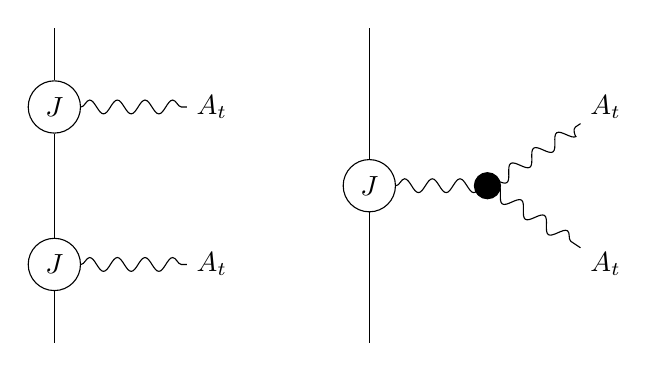
\begin{tikzpicture}
	\begin{scope}
		\node[circle, draw] (J1) at (0,1) {$J$};
		\node[circle, draw] (J2) at (0,-1) {$J$};
		\node (A1) at (2,1)  {$A_{t}$};
		\node (A2) at (2,-1)  {$A_{t}$};
		\draw[decorate, decoration={snake}] (J1) --(A1);
		\draw[decorate, decoration={snake}] (J2) --(A2);
		\draw (0,2) -- (J1) --(J2) -- (0,-2); 
	\end{scope}	
	\begin{scope}[shift={(4,0)}];
		\node[circle, draw] (J) at (0,0) {$J$};
		\node (A1) at (3,1)  {$A_{t}$};
		\node (A2) at (3,-1)  {$A_{t}$};
		\node[circle,draw,fill=black, minimum size = 0.2pt]  (V) at (1.5,0) {};  
		\draw[decorate, decoration={snake}] (J) -- (1.5,0) --  (A1);
		\draw[decorate, decoration={snake}] (1.5,0) --(A2);
		\draw (0,2) -- (J)-- (0,-2);
	\end{scope}
	\end{tikzpicture}
	\caption{Cancellation of the gauge anomaly of these two diagrams leads to the equation for the commutation relations involving the currents $J[k]$.
	\label{fig:cancel1}}
\end{figure}

$\bullet$
Next, let's consider the classical commutation relation 
\begin{equation}\label{eqn:rel2}
[J_a [k] , K_b [\ell]] = f_{ab}^c K_{c} [k+\ell]
\end{equation}

The BRST variation of the term \brian{write path integral above} in the path integral vanishes provided
\[
\int_t \sum_k \frac1{k!} \partial_z^k \left(f_{bc}^a \fc^b(t) B^c_t (t) \right) K_a[k] (t) = \int_t \sum_{\ell,m} \frac1{\ell!} \frac1{m!} \partial^\ell \fc^d (t) \partial^m B^e (t) [J_d (t), K_e(t)]  .
\] 
To obtain the commutation relation \eqref{eqn:rel2}, one sets 
\begin{align*}
B_t & = \ft_b z^{m} \delta_{t=0} \\
\fc & = \ft_a z^\ell .
\end{align*}

This commutation relation is equivalent to the cancellation of the gauge variation of the tree-level Feynman diagrams in Figure~\ref{fig:cancel2}.

\begin{figure}
	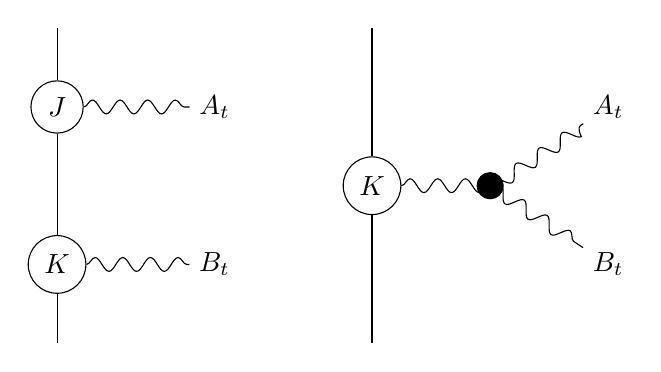
\begin{tikzpicture}
	\begin{scope}
		\node[circle, draw] (J1) at (0,1) {$J$};
		\node[circle, draw] (J2) at (0,-1) {$K$};
		\node (A1) at (2,1)  {$A_{t}$};
		\node (A2) at (2,-1)  {$B_{t}$};
		\draw[decorate, decoration={snake}] (J1) --(A1);
		\draw[decorate, decoration={snake}] (J2) --(A2);
		\draw (0,2) -- (J1) --(J2) -- (0,-2); 
	\end{scope}	
	\begin{scope}[shift={(4,0)}];
		\node[circle, draw] (J) at (0,0) {$K$};
		\node (A1) at (3,1)  {$A_{t}$};
		\node (A2) at (3,-1)  {$B_{t}$};
		\node[circle,draw,fill=black, minimum size = 0.2pt]  (V) at (1.5,0) {};  
		\draw[decorate, decoration={snake}] (J) -- (1.5,0) --  (A1);
		\draw[decorate, decoration={snake}] (1.5,0) --(A2);
		\draw (0,2) -- (J)-- (0,-2);
	\end{scope}
	\end{tikzpicture}
	\caption{Cancellation of the gauge anomaly of these two diagrams leads to the equation for the commutation relations involving $J[k]$ and $K[\ell]$.
	\label{fig:cancel2}}
\end{figure}

\subsection*{Quantum corrections}

We now turn to quantum corrections to the Koszul dual algebra.

The second diagram in Figure \ref{fig:cancel3} has a gauge anomaly.
We will show that this gauge anomaly is proportional to 
\[
\hbar \int_{\RR \times \{z=0\}} \partial_z \fc^a \kappa^{bc} f_{ab}^d J_{c} K_{d} + \cdots .
\]
The ellipses denote similar terms present in the anomaly which involve a higher number of holomorphic $z$-derivatives 

The second diagram in Figure \ref{fig:cancel4} also has a gauge anomaly.
We will show that this gauge anomaly is proportional to 
\[
\hbar \int_{\RR \times \{z=0\}} \partial_z \fc^a \kappa^{bc} f_{ab}^d K_{c} K_{d} + \cdots .
\]


\begin{figure}
	\begin{tikzpicture}
	\begin{scope}
		\node[circle, draw] (J) at (0,0) {$J$};
		%\node[circle, draw] (J2) at (0,-1) {$K$};
		\node (A) at (2,0)  {$A_{t}$};
		%\node (A2) at (2,-1)  {$B_{t}$};
		\draw[decorate, decoration={snake}] (J) --(A);
		%\draw[decorate, decoration={snake}] (J2) --(A2);
		\draw (0,2) -- (J) -- (0,-2); 
	\end{scope}	
	\begin{scope}[shift={(4,0)}];
		\node[circle, draw] (K) at (0,1) {$K$};
		\node[circle, draw] (J) at (0,-1) {$J$};
		\node (A) at (3,0)  {$A_{t}$};
		%\node (A2) at (3,-1)  {$B_{t}$};
		\node[circle,draw,fill=black, minimum size = 0.2pt]  (V) at (1.5,0) {};  
		\draw[decorate, decoration={snake}] (J) -- (1.5,0);
		\draw[decorate, decoration={snake}] (1.5,0) --(A);
		\draw[decorate, decoration={snake}] (K) -- (1.5,0);
		\draw (0,-2) -- (J) -- (K) -- (0,2);
	\end{scope}
	\end{tikzpicture}
	\caption{Cancellation of the gauge anomaly of these two diagrams leads to the $\hbar$-linear correction to the differential $\d J[k]$.
	\label{fig:cancel3}}
\end{figure}

\begin{figure}
	\begin{tikzpicture}
	\begin{scope}
		\node[circle, draw] (K) at (0,0) {$K$};
		%\node[circle, draw] (J2) at (0,-1) {$K$};
		\node (B) at (2,0)  {$B_{t}$};
		%\node (A2) at (2,-1)  {$B_{t}$};
		\draw[decorate, decoration={snake}] (K) --(B);
		%\draw[decorate, decoration={snake}] (J2) --(A2);
		\draw (0,2) -- (K) -- (0,-2); 
	\end{scope}	
	\begin{scope}[shift={(4,0)}];
		\node[circle, draw] (K1) at (0,1) {$K$};
		\node[circle, draw] (K2) at (0,-1) {$K$};
		\node (B) at (3,0)  {$B_{t}$};
		%\node (A2) at (3,-1)  {$B_{t}$};
		\node[circle,draw,fill=black, minimum size = 0.2pt]  (V) at (1.5,0) {};  
		\draw[decorate, decoration={snake}] (K1) -- (1.5,0);
		\draw[decorate, decoration={snake}] (1.5,0) --(B);
		\draw[decorate, decoration={snake}] (K2) -- (1.5,0);
		\draw (0,-2) -- (K2) -- (K1) -- (0,2);
	\end{scope}
	\end{tikzpicture}
	\caption{Cancellation of the gauge anomaly of these two diagrams leads to the $\hbar$-linear correction to the differential $\d K[k]$.
	\label{fig:cancel4}}
\end{figure}


\section{Koszul duality: an example of a free theory}

%\brian{renamed fields in terms of gauge theory above Let us step back and consider the free limit of the 3d gauge theory on $\RR \times \CC$. 
%Set $V = \fg$. 
%It will be useful to slightly rename the fields as $\phi = B$, $\psi_\zbar = A_{\zbar}$, and $\psi_t = A_t$ so that the free action reads
%}

We turn to a three-dimensional example. 
This theory is equivalent to the twist of the $3d$ $\cN=2$ chiral multiplet. 
The starting data is a complex vector space $V$.

First, we consider the theory defined on $\RR^3$. 
It will be convenient to choose coordinates of the form
\[
(t ; z) \in \RR_t \times \CC_z \simeq \RR^3
\]
where $t$ is a real coordinate along $\RR$ and $z$ is a holomorphic coordinate along the remaining $\CC \cong \RR^2$ direction. 

The fields consist of a scalar $\phi$ valued in $V$ and a partial one-form 
\[
\psi = \psi_t \d t + \psi_\zbar \d \zbar 
\]
valued in $V^*$. 
The free action reads
\[
\int \phi \partial_t \psi_\zbar + \int \phi \partial_\zbar \psi_t .
\]

The equations of motion for the scalar $\phi$ read
\begin{align*}
\frac{\partial}{\partial t} \phi & = 0 \\
\frac{\partial}{\partial \zbar} \phi & = 0 .
\end{align*}
The first equation implies that $\phi$ is constant in the $t$-direction and the second implies that $\phi$ is holomorphic in the variable $z$. 

The equation of motion for the one-form field $\psi$ reads
\[
\frac{\partial}{\partial t} \psi_\zbar - \frac{\partial}{\partial \zbar} \psi_t = 0 .
\]

There is an abelian gauge symmetry which acts on the $\psi$-fields as follows.
The gauge symmetry is given by a $V^*$-valued scalar $\chi$ which acts on the fields by
\begin{align*}
\delta \psi_t & = \frac{\partial}{\partial t} \chi \\
\delta \psi_\zbar & = \frac{\partial}{\partial \zbar} \chi .
\end{align*}

\subsection*{Local operators}

In this section we describe the algebra of local operators at $z = t = 0$ up to gauge equivalence.

The equations of motion imply that the $\phi$ has vanishing $t$ and $\zbar$-derivatives. 
Thus, the only local operators built from $\phi$ must be given by holomorphic $z$-derivatives. 
Let $V^*_{(n)} \simeq V^*$ denote the span of the local operators of the form $\partial_z^n \phi(0)$.
Thus, the linear local operators in $\phi$ span the vector space $\oplus_{n \geq 0} V_{(n)}^*$.
Since $\phi$ is a scalar, the algebra of operators involving only $\phi$ combine to form the symmetric algebra ${\rm S}^\bu \left(\oplus_{n \geq 0} V^*_{(n)}\right)$.

Next, consider local operators of the one-form field $\psi = \psi_t \d t + \psi_\zbar \d \zbar$. 
We claim that up to gauge equivalence there are no nontrivial local operators depending on $\psi_t, \psi_\zbar$.  
The easiest way to see this is to introduce the two-form field
\[
\d z \wedge \psi = \psi_t \d z \wedge \d t + \psi_\zbar \d z \wedge \d \zbar .
\]
Then, the equations of motion are equivalent to the condition that this two-form be closed for the de Rham differential
\[
\d \left(\d z \wedge \psi\right) = 0 .
\]
In other words, $\d z \wedge \psi \in Z^2 (\RR^3)$. 

Consider the one-form gauge symmetry $\d z \wedge \chi$. 
In this notation, the gauge symmetry simply reads $\delta (\d z \wedge \psi) = \d (\d z \wedge \chi)$. 
By a slight refinement of the Poincar\'{e} lemma for smooth differential forms, we can find one-form of the form $\d z \wedge \chi$ rendering $\d z \wedge \psi \in Z^2(\RR^3)$ gauge trivial. 

Finally, consider local operators built from the ghost field $\chi$. 
The gauge transformations preserving $\psi = 0$ satisfy $\frac{\partial}{\partial \zbar} \chi = \frac{\partial}{\partial t} \chi = 0$. 
Thus, similarly to $\phi$, the local operators one can build from $\chi$ only involve holomorphic $z$-derivatives. 
Let $V_{(n+1)} \simeq V$ denote the span of the local operators of the form $\partial_z^n \chi(0)$.
Thus, the linear local operators in $\chi$ span the vector space $\oplus_{n > 0} V_{(n)}$.
Since $\chi$ is a gauge symmetry, the algebra of operators involving only $\chi$ combine to form the exterior algebra $\wedge^\bu \left(\oplus_{n > 0} V_{(n)}\right)$. 
\footnote{More precisely, we obtain the {\em graded symmetric} algebra $\Sym(V_{(n)}[-1])$ of $V_{(n)}$ concentrated in degree $+1$.
We will only use the underlying $\ZZ/2$-graded vector space in this section.}

Summarizing our discussion thus far, we see that the local operators are of the form
%\[
%{\rm S}^\bu \left(z^{-1} V^*[z^{-1}]\right) \otimes \wedge^\bu \left(V[z^{-1}]\right)
%\]
%which we can slightly rewrite as
\[
\bigotimes_{n \geq 0} {\rm S}^\bu \big(V^*_{(n)}\big) \otimes \bigotimes_{m > 0} \wedge^\bu \big(V_{(m)}\big)
\]
where $V_{(n)}^* \simeq V^*$ indicates the vector space spanned by local operators of the form $\partial^n_{z} \phi(0)$ and $V_{(m+1)} \simeq V$ indicates the vector space spanned by local operators of the form $\partial^{m}_z \chi$. 

\subsection*{Character of local operators}

We contemplate the following two symmetries of the free theory.
The first corresponds to conformal symmetries along the $z$-plane. 
Concretely, consider the piece of this generated by $\U(1)$ rotations of $\CC_z$.
Infinitesimally, this is generated by the holomorphic vector field $z \frac{\partial}{\partial z}$. 

Second, there is a flavor symmetry.
Indeed, suppose that $V$ transforms according to some $G_f$ representation, where $G_f$ is the flavor group. 
Then we obtain a symmetry of this system by declaring that $\phi$ transform according to this representation and $\psi$ transform in the dual representation.

The character of the space of local operators is written in terms of fugacities $q$ and $u$ where $q$ is the fugacity of the $\U(1)$ conformal symmetry and $u$ is a vector in the maximal torus $T_f$ of the flavor group $G_f$. 
\[
\chi(q , u) = \frac{1}{|{\rm Weyl}(G)|} \oint_{s \in T_f} \frac{\d s}{2 \pi i s} \prod_{\alpha \in {\rm wt}(V)} (1-s_\alpha) \frac{(q s^{-1}_\alpha ; q)_\infty}{(s_\alpha ; q)_\infty} .
\]

\brian{If I break this $\U(1)_q \times G_f$ to $\U(1)_q \times \U(1)_s$ I can write the character as
\[
\prod_{n \geq 0} \frac{1 - s^{-1} q^{n+1}}{1 - s q^n} .
\]
}

\subsection*{Boundary conditions}

We extend the theory on $\RR \times \CC$ to a theory on $\RR \times \PP^1$ by choosing boundary conditions at $\infty \in \PP^1$.  
The boundary conditions we choose:
\begin{itemize}
\item the scalar $\phi$ vanishes at $\infty \in \PP^1$. 
That is, 
\[
\phi \in \Gamma \left(\RR \times \PP^1 \, , \, \cO(-1) \otimes V \right) .
\]
\item the components of the one-form $\psi_{t}, \psi_{\zbar}$ have simple poles at $\infty \in \PP^1$:
\[
\psi_{t}, \psi_{\zbar}\in \Gamma\left(\RR \times \PP^1 \, , \, \cO(1) \otimes V^*\right)
\]
\end{itemize}

Additionally, we must fix the boundary behavior of the gauge field $\chi$ to be compatible with the above choices.
A natural way to do this is to require the gauge field to acquire a simple pole at $\infty \in \PP^1$:
\[
\chi \in C^\infty\left(\RR \times \PP^1 \, , \, \cO(1) \otimes V^*\right) .
\]

\begin{lem}
The compactification of the theory along 
\[
\begin{tikzcd}
\RR \times \PP^1 \ar[d] \\ \RR
\end{tikzcd}
\]
results in the trivial one-dimensional theory. 
\end{lem}
\begin{proof}
The point is that every solution to the equations of motion is gauge equivalent to the trivial solution. 
For the scalar $\phi$, notice that the equations of motion require it to be constant along $\RR$ and holomorphic $\dbar \phi = 0$. 
Since there are no global holomorphic sections on $\PP^1$, we see that $\phi$ must be the trivial solution. 

The remaining equations of motion are
\[
\frac{\partial}{\partial \zbar} \psi_t - \frac{\partial}{\partial t} \psi_\zbar = 0 .
\]
\brian{finish} \footnote{In the BV language this follows from the fact that $\chi$ and $\psi$ comprise the cohomology $H^\bu(\PP^1, K_{\PP^1} \otimes \cO(1))\simeq 0$.}

%Again, $\psi_t$ is required to be constant along $\RR$ and be holomorphic $\dbar \psi_t = 0$. 

\end{proof}

%Two steps:
%\begin{itemize}
%\item There is a relation in the algebra of local operators of the form
%\[
%[B^b, B^c] = \hbar f^{bc}_a \partial_z B^a + O(\hbar^2)  .
%\]
%This gives rise to a term in the differential on the Koszul dual algebra of the form
%\[
%\d (z \ep \ft_a) = \hbar  f^{bc}_a (\ep \ft_b) \otimes (\ep \ft_c) + O(\hbar^2) .
%\]
%\item There is a relation in the algebra of local operators of the form
%\[
%[B^b, \fc^c] = \hbar f^{bc}_a \partial_z \fc^a + O(\hbar^2) .
%\]
%This gives rise to a term in the differential on the Koszul dual algebra of the form
%\[
%\d (z \ft_a) = \hbar  f^{bc}_a (\ep \ft_b) \otimes (\ft_c) + O(\hbar^2) .
%\]
%\brian{do I need to symmetrize?}
%\end{itemize}
\section{Higher dimensional defects} 

%higher dimensional topological defects. PSM in 3dCS. 
%Kapustin--Salina.
%Check refs by Mnev et al on BV-BFV?

\begin{thebibliography}{KWWY14}

\bibitem[MW97]{MW97}
G.~W.~Moore and E.~Witten,
``Integration over the u plane in Donaldson theory,''
Adv. Theor. Math. Phys. \textbf{1}, 298-387 (1997)
doi:10.4310/ATMP.1997.v1.n2.a7
[arXiv:hep-th/9709193 [hep-th]].

\bibitem[W88]{W88}
E.~Witten,
``Topological Quantum Field Theory,''
Commun. Math. Phys. \textbf{117}, 353 (1988)
doi:10.1007/BF01223371


\bibitem[WZ92]{WZ92}
E.~Witten and B.~Zwiebach,
``Algebraic structures and differential geometry in 2-D string theory,''
Nucl. Phys. B \textbf{377}, 55-112 (1992)
doi:10.1016/0550-3213(92)90018-7
[arXiv:hep-th/9201056 [hep-th]].


\end{thebibliography}

\end{document}